\section{Das Potenzial-Problem}

Im folgenden werde ich mich mit dem Potential-Problem beschäftigen.

\begin{mydef}\label{def_potential}
	Das Potential $k$ ist eine Art Kontostand, mit dem eine oder mehrere Kantengewichte reduziert werden können. Die Größe des Potentials gibt an, um wie viel die Gewichte insgesamt reduziert werden dürfen. Durch das Anwenden des Potentials soll sich die Anzahl der benötigten Agenten möglichst stark reduzieren.
\end{mydef}

Ich betrachte verschiedene, unterschiedlich komplizierte Varianten des Potential-Problems und werde für die jeweilige Variante einen Algorithmus angeben und kurz die Laufzeit begründen.

\subsection{Spezialfall $k = 1$}

In diesem Kapitel beschreibe ich das Potential-Problem $k = 1$. Dies bedeutet, dass auf genau einer beliebigen Kante das Kantengewicht um genau 1 reduzieren werden darf. Allerdings muss das Gewicht nach der Reduzierung  weiterhin $\geq 1$ sein. Ziel ist es, wie in Definition \ref{def_potential} beschrieben, die Anzahl der Agenten möglichst gut zu reduzieren.
\\
\\
Jeder Knoten berechnet im Algorithmus von \cite{cima_paper} die minimale Anzahl von Agenten (siehe Kapitel \ref{kap_algorithmus}) und es lässt sich schnell überlegen, dass die Höhe der Agentenanzahl an jedem Knoten von bestimmten Kanten mit ihren Gewichten abhängt.
\\
\\
Die Idee, um das Potenzial-Problem für den Spezialfall $k = 1$ zu lösen, ist nun, die Abhängigkeiten zu speichern, welche Kanten die Agentenzahl in jedem Knoten beeinflussen. Dazu protokollieren wir im modifizierten Algorithmus (aus Kapitel \ref{modifizierterAlgoChapter}), wie jede berechnete Nachricht zustande kommt, also von welchen Kanten sie abhängt.
\\
\\ 
Wie in der modifizierten Variante des Algorithmus beschrieben, kann man sehen, dass eine Nachricht $\lambda_{y}$ aus drei verschiedenen Fällen entstehen kann:

\begin{enumerate}[label=\alph*)]
	
	\item aus den beiden größten Kanten $\lambda_{y} \gets edge_{1} + edge_{2}$ \label{entstehung_nachricht_max1+max2}
	
	\item aus der Kante, über welche die Nachricht gerade verschickt wird (diese entspricht dem Knotengewicht) $\lambda_{y} \gets \omega(x)$
	
	\item aus der größten angekommenen Nachricht $\lambda_{y} \gets l_{1}$

\end{enumerate}

Je nachdem, durch welchen Fall eine Nachricht $\lambda_{y}$ berechnet wird, kommen andere Kanten in Frage, die wir protokollieren müssen.
Allerdings gilt für alle Fälle, dass wir uns maximal zwei Kanten merken müssen, da wir ansonsten die minimale Agentenzahl nicht verringern können. Gibt es keine oder mehr als zwei Kanten, so merken wir uns nur die Information, dass das Potential an dieser Stelle nicht eingesetzt werden kann, um die Agentenzahl zu reduzieren (wir setzen einen "flag").

\begin{theorem}\label{theorem_max2kanten}
	Es müssen maximal zwei Kanten pro Nachricht protokolliert werden. Ansonsten kann das Potential nicht angewendet werden und wir setzen eine "'flag"'
\end{theorem}

\begin{proof}[Widerspruchsbeweis]
	Wir nehmen an, es könnten mehr als zwei Kanten pro Nachricht protokolliert werden, o.B.d.A. drei Kanten. Dies würde bedeuten, dass wir durch Reduzierung einer dieser drei Kanten die Nachricht verkleinern könnten. Allerdings hängt die Berechnung der Nachricht pro Fall von maximal zwei Kanten ab (siehe den gerade genannten Fall \ref{entstehung_nachricht_max1+max2}). Dies bedeutet, dass die drei Kanten aus zwei verschiedenen Fällen stammen müssen. Wenn also nun eine der drei Kanten reduziert wird, kann sich maximal nur ein Fall verkleinern, der andere bleibt unverändert. Da der Fall ausschlaggebend ist, der die größte Nachricht generiert, wird durch die Reduzierung der Kante die Nachricht nicht verändert. Da wir aber gesagt haben, dass alle drei Kanten die Nachricht reduzieren können, ist dies ein Widerspruch dazu, dass eine Nachricht von mehr als zwei Nachrichten abhängen kann.
\end{proof}

Im folgenden werde ich bei allen drei möglichen Fällen beschreiben, welche Kanten unter welcher Bedingung protokolliert werden. Um protokollieren zu können, wird die Nachricht (siehe Definition \ref{def_nachricht}) etwas erweitert. Sie enthält nun nicht mehr nur die Anzahl der Agenten, die für den Teilbaum benötigt werden, sondern auch die (bis zu) zwei protokollierten Kanten bzw. einen "flag", falls keine eindeutigen Kanten bestimmt werden konnten.

\begin{enumerate}[label=\alph*)]
	
	\item In diesem ersten Fall wird die Nachricht aus den beiden größten Kanten berechnet ($\lambda_{y} \gets edge_{1} + edge_{2}$). Allerdings müssen wir kontrollieren, ob diese zwei Kanten eindeutig sind, oder ob es evtl. mehrere gleich große Kanten gibt. Ist die Wahl der Kanten nicht eindeutig, müssen wir dies bei der Protokollierung mit berücksichtigen:\\
	
		\begin{algorithmic}
			\If {$edge_{1} == edge_{3}$}
			\State \uline{protokolliere} "flag"
			\State//Es gibt drei gleich große Kanten. Selbst wenn man eine Kante reduziert, wird die Nachricht aus den anderen beiden Kanten berechnet und dadurch nicht reduziert.
			\ElsIf {$edge_{2} == edge_{3}$}
			\State \uline{protokolliere} $edge_{1}$
			\State//Die maximale Kante ist eindeutig, die zweit größte nicht. Es macht also nur Sinn die größte zu reduzieren.
			\Else
			\State \uline{protokolliere} $edge_{1}$ und $edge_{2}$
			\State//Sowohl die größte, als auch die zweit größte Kante ist eindeutig. Wir können eine von den beiden reduzieren, um auch die Nachricht erfolgreich zu reduzieren.
			\EndIf
		\end{algorithmic}
	
	\item Die Nachricht ist kleiner als das Knotengewicht: $\omega(x) \geq edge_{1}+edge_{2}$. Da aber $\omega(x)$ so definiert ist, dass es den Wert des größten Kantengewicht inzident zu x hat, muss die Kante ausschlaggebend sein, über die die Nachricht verschickt wird. 
	\\
	Diese Kante zwischen x und y ist für den Nachrichtenwert also entscheidend und wird somit in der Nachricht protokolliert: \uline{Protokolliere} Kante zwischen x und y.
	
	\item In diesem Fall bestimmt die größte ankommende Nachricht $l_{1}$ die neu berechnete Nachricht. Da keine weitere Kante mehr Einfluss genommen hat, übernehmen wir die protokollierten Kanten (oder die "flag") aus $l_{1}$ für $\lambda_{y}$: \uline{Protokolliere} das gleiche wie $l_{1}$
	
\end{enumerate}
Man muss noch beachten, dass mehrere Fälle gleichzeitig auftreten können. Passiert dies, muss man einen weiteren Test durchführen, ob die verschiedenen Fälle unterschiedlich protokollieren würden.
\\
Würden die Fälle verschieden protokollieren, so protokolliere "flag", da das Potenzial an dieser Stelle nicht genutzt werden kann, ansonsten behalte die Protokollierung bei.

\subsection{Potenzial auf einer Kante mit $k \geq 1$}


Um das Potential-Problem etwas zu erweitern, betrachte ich im folgenden Abschnitt Potenziale $\geq 1$, allerdings mit der Einschränkung, dass man das gesamte Potenzial k nur auf einer Kante einsetzen darf.

\begin{theorem}
	Man kann trotz beliebig großen Potential nicht garantieren, dass sich die minimale Anzahl an benötigten Agenten reduziert, wenn das Potential nur auf einer Kante eingesetzt werden darf.
\end{theorem}

\begin{proof}[Widerspruchsbeweis]
	Annahme: Es sei mit beliebig großem Potential immer möglich, die Anzahl der benötigten Agenten zu reduzieren.
	
	\begin{figure}[hbt]
		\subfigure[alle Kanten haben Gewicht 4. Alle Knoten benötigen mindestens 8 Agenten.]{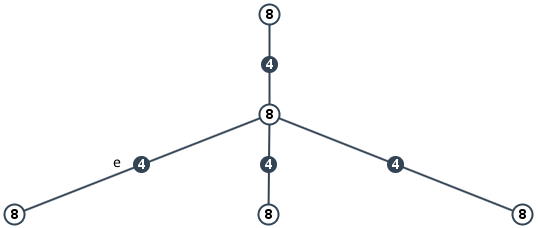
\includegraphics[width=0.65\textwidth]{bilder/abb1.png}} 
%		\hfill

		\subfigure[eine Kante wurde auf Gewicht 1 geduziert, alle anderen haben weiterhin Gewicht 4. Alle Knoten benötigen trotzdem mindestens 8 Agenten.]{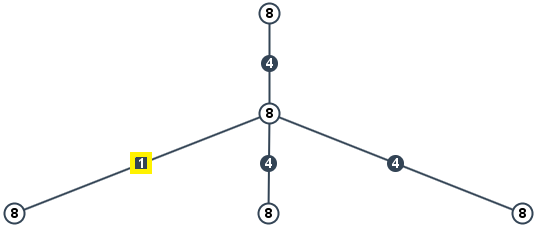
\includegraphics[width=0.65\textwidth]{bilder/abb2.png}} 
		\caption{Beispiel, dass Verringerung auf einer Kante nicht zu einer Verringerung der notwendigen Agenten führen muss} 
		\label{abb_gegenbeispielMaxPotential}
	\end{figure} 
	
	
	Da das Potenzial k beliebig groß ist, kann man die Kante, auf welche man das Potential anwenden möchte, auf Kantengewicht 1 setzen. Dadurch kann man garantieren, dass das größtmögliche Potential eingesetzt worden ist (jede Kante muss immer ein Gewicht $\geq 1$ haben). Trotzdem ist es nicht möglich bei folgendem Baum die Anzahl der Agenten zu reduzieren (siehe Abbildung \ref{abb_gegenbeispielMaxPotential}).
	\\
	\\
	Dies ist ein Widerspruch zur Annahme, dass man die Agentenanzahl auf einem beliebigen Baum mit beliebig großem Potential immer reduzieren kann.
\end{proof}

Trotzdem ist es möglich einen Algorithmus anzugeben, der die Kante auswählt, welche die Agentenanzahl am meisten minimiert, falls es eine solche Kante gibt.


\subsection*{Algorithmus Idee}

	Auch um dieses Problem zu lösen, muss die in Kaptiel \ref{modifizierterAlgoChapter} benutze Nachricht angepasst werden. Die Idee dieses Algorithmus ist es - ähnlich wie beim Spezialfall $k = 1$ -  Protokoll zu führen. Damit lässt sich im Anschluss bestimmen, welche Kante am sinnvollsten reduziert werden muss.\\
	Die Idee ist es für jeden Knoten folgende Dinge festzuhalten: 
	\begin{itemize}
		\item $\mu$: die normale Agentenanzahl (wird wie in Kapitel \ref{modifizierterAlgoChapter} ganz normal berechnet).
		\item $\hat{\mu}$: die benötigte Anzahl an  Agenten, die durch die maximal mögliche Reduzierung bis zu diesem Zeitpunkt erreicht werden kann.
		\item $e_{1} / e_{2}$: die Kanten, die reduziert wurden.
	\end{itemize}
	Hat jeder Knoten am Ende des Algorithmus diese Informationen, kann man mit einem Durchlauf durch alle Knoten das Minimum ermitteln. Da außerdem gespeichert ist, welche Kanten dafür reduziert werden müssen, sind kann man auf eine dieser Kanten das Potential anwenden, um die Agentenzahl entsprechend zu reduzieren. Wie in Theorem \ref{theorem_max2kanten} argumentiert, kommen immer nur maximal zwei Kanten pro Knoten in Frage.
	
	\subsection*{Berechnung der Nachricht}
	
	Um diese Informationen zu generieren, müssen die Nachrichten erweitert werden.
	Diese enthalten nun mehrere Parameter:
	\begin{itemize}
		\item $\alpha$: die normal berechnete Nachricht (siehe Kapitel \ref{modifizierterAlgoChapter})
		\item $\beta$: modifizierte Nachricht (,die durch das Potential am stärksten reduzierte Nachricht)
		\item $e_{1} / e_{2}$: die Kanten, auf die das Potential angewendet worden ist
	\end{itemize}
	Es bleibt noch zu klären, wie die modifizierte Nachricht $\beta$ und die Kanten $e_{1}$ und $e_{2}$ berechnet werden:\\
	Es gibt bis zu vier Kanten, auf die das Potential pro Nachricht angewendet werden kann, um die richtige modifizierte Nachricht zu generieren. Daher muss das Potential nacheinander auf allen in Frage kommenden Kanten angewendet werden. Die Kante, die die größte Reduzierung zur Folge hat, wird neben dem veränderten Wert mit in die Nachricht gespeichert. \\
	Wir gehen alle Fälle durch, um die modifizierte Nachricht $\beta$ von Knoten x nach y zu berechnen:
	\begin{enumerate}
		\item berechnet $\beta$, indem das Potential auf die Kante zwischen x und y angewendet wird ($edge_{xy} - potential$).
		\item berechnet $\beta$, indem das Potential auf die größte Kante $edge_{1}$ angewendet wird ($edge_{1} - potential$) .
		\item berechnet $\beta$, indem das Potential auf die zweitgrößte Kante $edge_{2}$ angewendet wird ($edge_{2} - potential$).
		\item berechnet $\beta$, indem aus $l_{1}$ nicht die normale Nachricht $\alpha$, sondern die modifizierte Nachricht $\beta$ verwendet wird.
	\end{enumerate}
	Der kleinste $\beta$-Wert aus diesen vier Fällen ist unsere modifizierte Nachricht. Die Kanten, auf die das Potential angewendet wurde, wird als 3. Parameter $e_{1} / e_{2}$ in der Nachricht mit verschickt.
	\\
	\\
	Diese Nachrichten werden wie im normalen Algorithmus (Kapitel \ref{kap_algorithmus}) zwischen allen Knoten verschickt, bis jeder Knoten von jedem Nachbar genau eine Nachricht bekommen hat.
	
	
	\subsection*{Berechnung der minimalen Agenten ($\mu$)}
	
	Um nun das $\hat{\mu}$ jedes Knotens zu berechnen, gehen wir analog zur Berechnung der Nachricht vor. Der einzige Unterschied ist, dass es einen Fall weniger gibt: 
	\begin{enumerate}
		\item berechnet $\hat{\mu}$, indem das Potential auf die größte Kante $edge_{1}$ angewendet wird ($edge_{1} - potential$) .
		\item berechnet $\hat{\mu}$, indem das Potential auf die zweitgrößte Kante $edge_{2}$ angewendet wird ($edge_{2} - potential$).
		\item berechnet $\hat{\mu}$, indem aus $l_{1}$ nicht die normale Nachricht $\alpha$, sondern die modifizierte Nachricht $\beta$ verwendet wird.
	\end{enumerate}
	Da wir keine Nachricht mehr verschicken müssen, sondern nur noch das $\hat{\mu}$ ausrechnen wollen, gibt es keine Kante mehr, über die eine Nachricht verschickt wird. Ansonsten sind die Fälle mit der Nachrichtenberechnung identisch.\\
	Nachdem wir für jeden Knoten die drei Parameter ausgerechnet haben, wissen wir für jeden Knoten wie viele Agenten wir brauchen, wenn wir das Potential nicht anwenden (das ganz normale $\mu$); wie viele Agenten wir benötigen, wenn wir das Potential anwenden $\hat{\mu}$; und auf welche Kanten wir das Potential anwenden müssen, um diese Verbesserung zu erreichen (die Kanten, die wir zur Berechnung von $\hat{\mu}$ reduziert haben).\\
	Durch einen linearen Durchlauf durch alle Knoten können wir nun das Minimum berechnen und die dazugehörige Kante auswählen, auf die das Potential angewendet werden muss.
	\begin{theorem}
		Die Berechnung aller Nachrichten und die Bestimmung der Kante, auf die das Potential angewendet werden sollte, ist in linearer Laufzeit möglich.
	\end{theorem}
	\begin{proof}
		Analog zu Theorem \ref{thm_laufzeit_modifikation} wird die Grundidee des Algorithmus nicht verändert. Jeder Knoten schickt zu all seinen Nachbarn je eine Nachricht. Die Anzahl der Nachrichten ändert sich durch die Modifikation nicht, sondern nur die Berechnung an sich.\\Die Berechnung kann auch hier in konstanter Zeit durchgeführt werden, da pro Nachricht nur maximal vier konstante Fälle berechnet werden muss und aus diesen das Minimum bestimmt werden muss.
	\end{proof}
	TODO:\\
	//begründung korrektheit

\subsection{Potenzial verteilen mit k > 1}